% Geometry, font
\documentclass[12pt, letter]{article}
\usepackage[margin=0.8in]{geometry}
\usepackage[T1]{fontenc}
\usepackage{fourier}
\usepackage{titling}
\setlength{\droptitle}{-5em} 
\usepackage[parfill]{parskip}
\usepackage{graphicx}
\graphicspath{{imgs/}}
\usepackage{hyperref}

% Math stuff
\usepackage{amssymb}
\usepackage{bm}

% Code Highlighting
\usepackage{minted}
\usemintedstyle{solarizedlight}

\author{Zach Neveu}
\title{ Day 13 Notes }

\begin{document}
\maketitle

\section{Agenda}%
\label{sec:agenda}
\begin{itemize}
	\item ILP Advanced Techniques
	\item Project 3
	\item Intro to Branch \& Bound
	\item TODO:
	\begin{itemize}
		\item Reading
		\item HW due Tomorrow
		\item Project due Monday
		\item Quiz next Tuesday
	\end{itemize}
\end{itemize}

\section{ILP}%
\label{sec:ilp}
\begin{gather*}
3x_1+2x_2 \le 18 \\
OR \\
x_1+4x_2 \le 16
\end{gather*}
\begin{itemize}
    \item Binary variables $x_1, x_2$
	\item How can we phrase this in terms of ILP?
	\item Typically, both would need to be solved
	\item Add a large number multiplied by a new binary variable
	\item Negate new variable in one equation so that this variable can control
	\item Now at least one constraint must be satisfied, or both can be satisfied
\end{itemize}

\begin{gather*}
3x_1+2x_2 \le 18 + yM, M \rightarrow \infty \\
x_1+4x_2 \le 16 + (1-y)M
\end{gather*}

\begin{itemize}
	\item Say we have three constraints now
	\item How to implement or with more than 3 inputs?
	\item Add 3 new variables
	\item Add constraint that 3 variables sum to less than 3
\end{itemize}
\begin{gather*}
3x_1+2x_2 \le 18 + y_1M \\
x_1+4x_2 \le 16 +y_2M\\
2x_1+3x_2 \le 14 +y_3M\\
y_1+y_2+y_3 \le 2\\
\end{gather*}

\section{Branch \& Bound}%
\label{sec:branch_&_bound}
\begin{itemize}
	\item Useful for solving ILP
	\item Also very useful for other stuff
	\item Based on divide and conquer
	\item In \ref{fig:bandb}, $x_0=(1.5, 2.5)$ is the solution to the LP relaxation of this problem.
	\item $x_0$ is non-integral, so we keep going
	\item Subdivide the feasible region into two non-overlapping feasible regions such that no feasible solutions are excluded.
	\item SP1: add constraint $x \le 1$
	\item SP2: add constraint $x \ge 2$
	\item Keep subdividing on integer boundaries
	\item for SP1: add $y\le 1$ SP3, add $y \ge 2$ SP4
	\item For SP2: add $\y \le 1$ SP5, $y\ge 2$ SP6
	\item SP4, SP6 infeasible, no points in those areas
	\item Find LP solns to SP3, SP5
	\item LP soln to SP3 turns out to be integral - no need to keep going
	\item For SP5, add $x \le 2$ SP7, and $x \ge 3$ SP8
	\item SP8 infeasible
	\item SP7 has integral soln
	\item Compare integral solutions to SP7 and SP3
	\item No subproblems left to expand, choose best LP soln (SP7)
\end{itemize}

\begin{figure}[h]
	\centering
	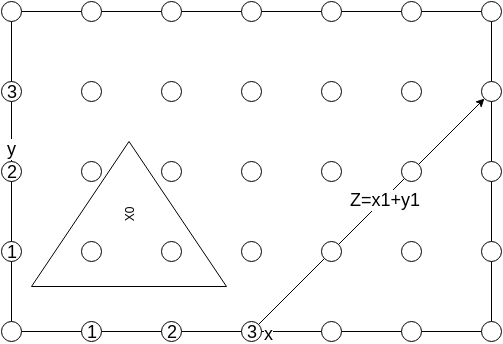
\includegraphics[width=0.8\textwidth]{bandb}
	\caption{ILP w/ Branch and Bound Example}
	\label{fig:bandb}
\end{figure}

\section{Project}%
\label{sec:project}
\begin{itemize}
	\item Solve knapsack and coloring using ILP
	\item Instances all converted already
	\item Must solve formulation of problem
	\item Turn in model files, output files
	\item Limit solver runtime to 10 minutes
\end{itemize}

\end{document}
